\documentclass[11pt,a4paper]{article}

% ---------------------------------------------------------------
% Packages
% ---------------------------------------------------------------
\IfFileExists{acl.sty}{
  \usepackage[final]{acl}
}{
  \usepackage[margin=2.5cm]{geometry}
}
\usepackage{times}
\usepackage{graphicx}
\usepackage{booktabs}
\usepackage{amsmath}
\usepackage{hyperref}
\usepackage{subcaption}
\usepackage{microtype}
\usepackage{enumitem}
\usepackage{xcolor}
\usepackage{placeins}

\hypersetup{colorlinks=true, linkcolor=black, citecolor=black, urlcolor=blue}

% ---------------------------------------------------------------
% Title block
% ---------------------------------------------------------------
\title{\textbf{Comparing Dijkstra, A*, and JPS4 on 4-Connected Grid Maps}\\[4pt]
\large Algorithm Design \& Analysis Final Project Report}

\author{
  Jazib Waqas \quad Salman Adnan \quad Hunain Abbas \\
  \texttt{jw08048 \quad sa07885 \quad sh08466}
}

\date{Spring 2026}

\begin{document}
\maketitle

% ---------------------------------------------------------------
\begin{abstract}
We compare three shortest-path algorithms on 4-connected grid maps: Dijkstra's algorithm, A*, and JPS4, a recent version of Jump Point Search for 4-directional movement. All three should find shortest paths in this setting, so the main question is how much work each one needs to find the same answer. We ran 30 trials per density level from 10\% to 40\% obstacle density on both 50$\times$50 and 100$\times$100 grids, for 420 problem instances per grid size. JPS4 expanded the fewest nodes in every tested case. It was also faster in most cases, but the time difference was smaller than the expansion difference because JPS4 does more work inside each step than normal A*. We also connected the pathfinders to a Snake demo so the algorithms can be seen on the same board, not only compared in tables.
\end{abstract}

% ---------------------------------------------------------------
\section{Introduction}

Shortest-path search on grid maps is a common operation in game AI, robotics, and navigation systems. The choice of algorithm matters in practice because a tile-based game may call a pathfinder many times during play, and a slow search can quickly become visible to the player.

This project targets a specific, well-defined setting: a 4-connected grid where every step costs 1. That constraint rules out 8-directional movement, weighted edges, and any-angle paths. Within those boundaries, we compare three algorithms that all find optimal paths:

\begin{itemize}[nosep]
  \item \textbf{Dijkstra}: the uninformed baseline. It has no heuristic and expands outward in distance order.
  \item \textbf{A*}: adds Manhattan distance as a heuristic to guide search toward the goal.
  \item \textbf{JPS4}: applies the 4-connected Jump Point Search idea from Baum (2025), using jump points to avoid expanding some unnecessary cells.
\end{itemize}

The core research question is simple: does JPS4 give a useful advantage over A*, and when does it help most?

We built our own implementations of all three algorithms, wrote a test suite that checks path-length agreement across algorithms on hundreds of random instances, and ran a controlled benchmark across two grid sizes and seven density levels. The same code drives an interactive Snake demo where the algorithms can be watched side-by-side.

% ---------------------------------------------------------------
\section{Problem Definition}

The problem studied in this project is shortest-path search on a 4-connected grid. Each grid cell is either free or blocked. A valid move goes one cell up, down, left, or right, and every valid move has cost 1. The goal is to return a shortest path from a start cell to a target cell when a path exists.

This problem is simple enough to implement and test fully, but it still shows a real difference between the algorithms. Dijkstra, A*, and JPS4 should all return the same shortest path length, but they search the grid in different ways. Dijkstra uses no goal information. A* uses Manhattan distance to move the search toward the goal. JPS4 keeps the shortest-path guarantee while trying to skip cells that do not need to be expanded.

Our project measures this difference instead of only describing it. We compare node expansions, search time, and path lengths. We also use the Snake demo as a practical check that the pathfinders can be called repeatedly inside an interactive program.

% ---------------------------------------------------------------
\section{Background}

\subsection{Dijkstra's Algorithm}

Dijkstra (1959) finds shortest paths in graphs with non-negative edge costs by expanding nodes in order of their distance from the start~\cite{dijkstra1959}. On our grid, it behaves like a wave moving outward from the start. It is correct, but it has no idea where the goal is, so it can explore a large part of the reachable area before stopping.

\subsection{A* Search}

Hart, Nilsson, and Raphael (1968) add a heuristic estimate $h(n)$ of the remaining distance to the goal~\cite{hart1968}. The node priority becomes $f(n) = g(n) + h(n)$, where $g(n)$ is the true cost from the start. If the heuristic never overestimates, A* still finds a shortest path and usually expands fewer nodes than Dijkstra.

On a 4-connected grid with unit costs, Manhattan distance is the standard admissible heuristic:
\[
  h(n) = |x_n - x_{\text{goal}}| + |y_n - y_{\text{goal}}|
\]

\subsection{Jump Point Search and JPS4}

Jump Point Search (JPS), introduced by Harabor and Grastien (2011) for 8-connected grids, reduces a different kind of extra work~\cite{harabor2011}. Even with a good heuristic, A* can still check many paths that are basically the same length and shape. JPS tries to skip the repeated middle cells and jump to the important cells, called jump points.

Baum (2025) adapted this idea to 4-connected grids, producing JPS4~\cite{baum2025}. Since there is no diagonal movement, JPS4 uses different rules from the original JPS. In simple terms, it follows straight moves when possible and only stops when an obstacle or the goal makes a cell important to check.

This lets JPS4 skip some cells instead of expanding every cell one by one. The downside is that each JPS4 step is more complicated than A*'s normal 4-neighbor check.

% ---------------------------------------------------------------
\section{Methodology}

\subsection{Core Algorithms}

All three algorithms are implemented in \texttt{pathing\_grid.py} using a shared priority queue loop from \texttt{helper.py}. This keeps the code easier to compare because the algorithms mainly differ in how they choose the next cells:

\begin{itemize}[nosep]
  \item \textbf{Dijkstra} uses the same 4-neighbor expansion as A*, but uses a zero heuristic, so nodes are processed only by distance from the start.
  \item \textbf{A*} uses Manhattan distance as the heuristic and expands all 4 passable neighbors at each step.
  \item \textbf{JPS4} first removes some directions that do not need to be checked, then jumps along the remaining directions until it reaches a jump point, obstacle, or the goal.
\end{itemize}

JPS4 returns jump points directly. After the search finishes, the code fills in the skipped cells so the final output is still a normal cell-by-cell path.

\subsection{Grid and Connectivity}

The grid is a 2D Boolean array where \texttt{True} means blocked. The \texttt{PathingGrid} class also stores a Union--Find structure over free cells. This lets the code quickly check whether the start and goal are connected before running a search.

\subsection{Snake Demo}

The same \texttt{PathingGrid} is used in an interactive Snake game built in Tkinter. The game runs three rounds on the same frozen board, one per algorithm, and shows each algorithm's search time, expansion count, and path length below the grid. This makes the comparison easier to see because the board is the same for all three algorithms.

When the current food cell becomes temporarily unreachable because of the snake's body, the game falls back to a tail-following recovery strategy and relocates food to a reachable cell. This was added after testing showed that the pathfinder could be correct while the game loop still got stuck on unreachable food.

\subsection{Test Suite}

The test suite in \texttt{tests/} covers four properties:

\begin{enumerate}[nosep]
  \item \textbf{Path length agreement:} Dijkstra, A*, and JPS4 return the same path length on every solvable instance sampled.
  \item \textbf{Expansion ordering:} Dijkstra never expands fewer nodes than A* on the same instance. This checks that the heuristic is helping.
  \item \textbf{Reachable food selection:} the snake's food placement always picks a cell reachable from the snake's current head.
  \item \textbf{Recovery correctness:} the unreachable-food loop that appeared earlier no longer occurs.
\end{enumerate}

The current codebase passes all seven pytest tests.

% ---------------------------------------------------------------
\subsection{Benchmark Setup}

\subsubsection{Grid Generation}

The benchmark grids are generated randomly. For each trial, every cell is blocked with probability $\rho$, which is the obstacle density. We use two grid sizes: 50$\times$50 and 100$\times$100.

Start and goal cells are chosen to make the path reasonably long. We first pick a random free cell, run BFS to find the farthest reachable cell from it (call it $A$), then run BFS again from $A$ to find another farthest cell (call it $B$). The trial uses $A$ as start and $B$ as goal. This avoids very short path queries, which would not show much difference between the algorithms.

Each trial is run with all three algorithms on the same board. This controls for instance difficulty and lets us compare algorithms on identical queries.

\subsubsection{Parameters}

\begin{itemize}[nosep]
  \item \textbf{Grid sizes:} 50$\times$50 and 100$\times$100.
  \item \textbf{Density levels:} 0.10, 0.15, 0.20, 0.25, 0.30, 0.35, 0.40.
  \item \textbf{Trials per condition:} 30.
  \item \textbf{Seed:} fixed per density level (seed $= 99 + 7777 \times i + W$), so the benchmark can be repeated.
  \item \textbf{Metric: expansions.} The number of nodes popped from the priority queue. This is our main metric because it depends less on the computer than timing does.
  \item \textbf{Metric: time.} Python \texttt{time.perf\_counter} search time in milliseconds. These numbers are useful, but they are more affected by the machine and Python runtime.
\end{itemize}

Instances where any algorithm fails to find a path are excluded from that trial (none occurred in this study; the Union--Find pre-filter ensures we only run solvable instances).

% ---------------------------------------------------------------
\section{Results}

\subsection{Node Expansions}

Table~\ref{tab:expansions50} and Table~\ref{tab:expansions100} report mean expansion counts across densities for both grid sizes. Figure~\ref{fig:results50} and Figure~\ref{fig:results100} show the full sweep visually.

\begin{table*}[!t]
\centering
\caption{Mean node expansions on the 50$\times$50 grid (30 trials per density).}
\label{tab:expansions50}
\small
\begin{tabular}{lrrrrrrr}
\toprule
Algorithm & $\rho=0.10$ & $\rho=0.15$ & $\rho=0.20$ & $\rho=0.25$ & $\rho=0.30$ & $\rho=0.35$ & $\rho=0.40$ \\
\midrule
Dijkstra  & 2247.5 & 2121.6 & 1997.2 & 1858.6 & 1642.7 & 1241.7 &  624.3 \\
A*        & 1949.7 & 1628.5 & 1352.5 & 1118.3 &  898.2 &  823.5 &  463.5 \\
JPS4      &  570.5 &  639.2 &  627.5 &  590.7 &  512.6 &  497.0 &  281.7 \\
\bottomrule
\end{tabular}
\end{table*}

\begin{table*}[!t]
\centering
\caption{Mean node expansions on the 100$\times$100 grid (30 trials per density).}
\label{tab:expansions100}
\small
\begin{tabular}{lrrrrrrr}
\toprule
Algorithm & $\rho=0.10$ & $\rho=0.15$ & $\rho=0.20$ & $\rho=0.25$ & $\rho=0.30$ & $\rho=0.35$ & $\rho=0.40$ \\
\midrule
Dijkstra  & 8987.8 & 8490.4 & 7966.0 & 7434.1 & 6842.0 & 5605.7 & 2314.8 \\
A*        & 7903.1 & 6439.7 & 5334.5 & 3839.3 & 3881.2 & 3493.8 & 1870.8 \\
JPS4      & 2379.0 & 2500.1 & 2491.0 & 2031.6 & 2286.3 & 2103.4 & 1137.1 \\
\bottomrule
\end{tabular}
\end{table*}

\begin{figure*}[!t]
  \centering
  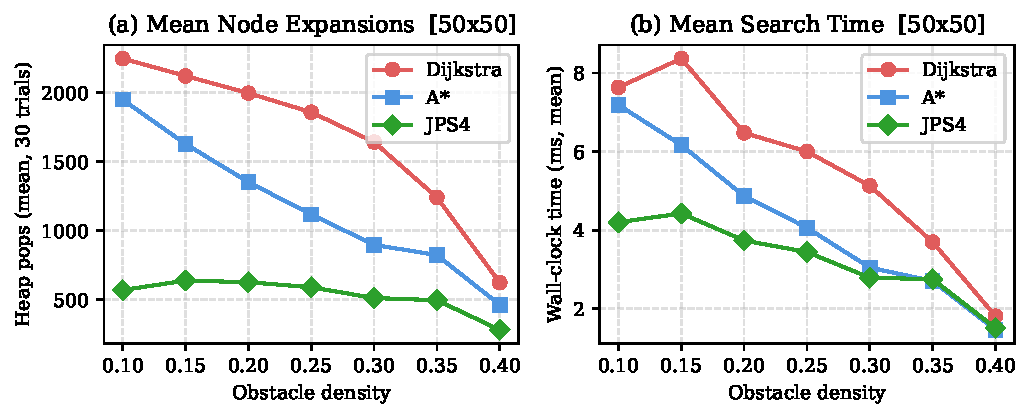
\includegraphics[width=\textwidth]{figures/results_50x50.pdf}
  \caption{Mean expansions (left) and mean wall-clock time (right) on the 50$\times$50 grid across seven density levels. Each point is the mean over 30 trials.}
  \label{fig:results50}
\end{figure*}

\begin{figure*}[!t]
  \centering
  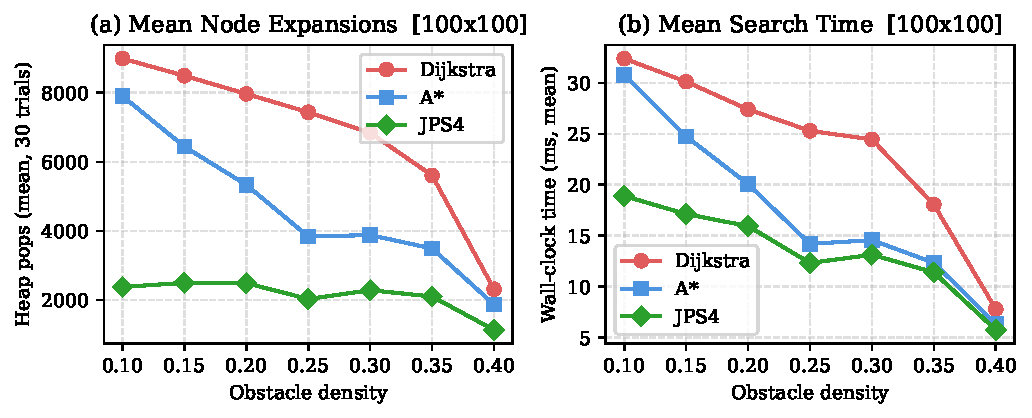
\includegraphics[width=\textwidth]{figures/results_100x100.pdf}
  \caption{Same metrics on the 100$\times$100 grid. The separation between JPS4 and the other two algorithms is more pronounced at this scale.}
  \label{fig:results100}
\end{figure*}

JPS4 expands the fewest nodes at every density level on both grid sizes. On the 100$\times$100 grid at $\rho = 0.10$, JPS4 expands 2,379 nodes, compared with 8,988 for Dijkstra and 7,903 for A*. This is a 73\% reduction compared with Dijkstra and a 70\% reduction compared with A*. In our benchmark, the low-density case helps JPS4 because the start and goal are far apart and there are many repeated grid patterns that JPS4 can skip.

At higher densities the gap becomes smaller. With more obstacles, paths turn more often and straight open areas are shorter, so JPS4 has fewer chances to jump. At $\rho = 0.40$ on the 100$\times$100 grid, JPS4 still reduces expansions by 51\% compared with Dijkstra and 39\% compared with A*, but the advantage is smaller than at low density.

Figure~\ref{fig:ratio} shows the expansion ratio relative to Dijkstra across both grid sizes, and Figure~\ref{fig:speedup} isolates JPS4's advantage over A*.

\begin{figure*}[!t]
  \centering
  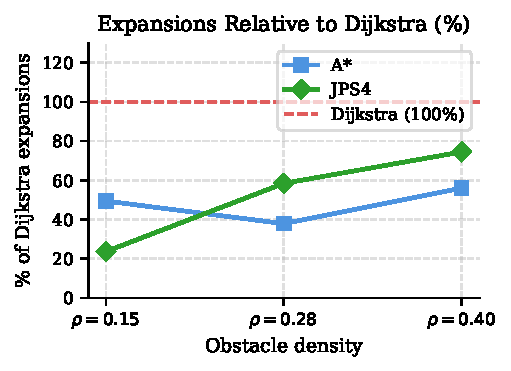
\includegraphics[width=\textwidth]{figures/expansion_ratio.pdf}
  \caption{Node expansions of A* and JPS4 expressed as a percentage of Dijkstra's count. Values below 100\% mean fewer expansions than Dijkstra. JPS4 is consistently the lowest.}
  \label{fig:ratio}
\end{figure*}

\begin{figure*}[!t]
  \centering
  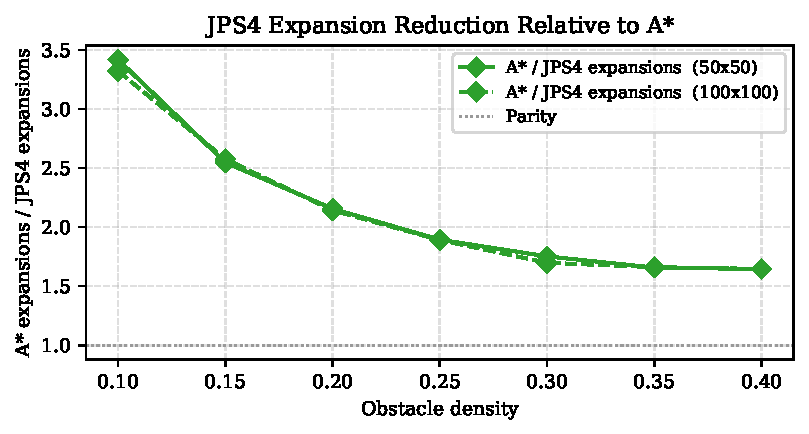
\includegraphics[width=0.7\textwidth]{figures/jps4_speedup.pdf}
  \caption{Ratio of A* expansions to JPS4 expansions. Values above 1.0 mean JPS4 expanded fewer nodes. The 100$\times$100 grid shows consistently larger gains.}
  \label{fig:speedup}
\end{figure*}

\subsection{Wall-Clock Time}

Search time follows the same general pattern as expansions, but it is noisier. On the 50$\times$50 grid, Dijkstra runs in roughly 6--8 ms at low density, A* in 4--6 ms, and JPS4 in 3--4 ms. The time gap is smaller than the expansion gap because JPS4's jump logic is more expensive per step than A*'s simple 4-neighbor lookup.

At $\rho = 0.35$ on the 50$\times$50 grid, JPS4 and A* have almost the same runtime, 2.75 ms versus 2.70 ms, even though JPS4 expands 40\% fewer nodes. This shows the cost of the extra JPS4 logic: each JPS4 step scans along a direction until it hits an obstacle or a forced neighbor.

On the 100$\times$100 grid, JPS4's time advantage becomes clearer again. At $\rho = 0.10$, JPS4 takes 18.9 ms, compared with 30.8 ms for A* and 32.4 ms for Dijkstra. On a larger grid, skipping long parts of the path saves enough work to make the extra JPS4 logic worthwhile.

\subsection{Path Correctness}

Every trial confirmed that all three algorithms return the same path length. This is expected, but it is still an important check because JPS4 is more complex than A*. The test suite also checks 500 random instances each run, and we did not find any path-length disagreements after the JPS4 implementation was finalized.

% ---------------------------------------------------------------
\section{Discussion}

\subsection{When JPS4 Helps Most}

The data in our benchmark shows JPS4's advantage is largest on:
\begin{itemize}[nosep]
  \item \textbf{Larger grids.} The 100$\times$100 grid sees bigger relative gains than 50$\times$50 at every density. Larger maps give the pruning more room to matter.
  \item \textbf{Lower obstacle density in our setup.} Our farthest-point start and goal selection creates long open searches at low density, and JPS4 benefits from that. At $\rho = 0.10$ on 100$\times$100, JPS4 expands 3.4$\times$ fewer nodes than Dijkstra.
\end{itemize}

\subsection{When JPS4 Helps Less}

At high density ($\rho \geq 0.35$), paths turn more often and there are fewer useful jumps. JPS4 still expands fewer nodes, but on smaller grids the extra work per step makes the time gap much smaller. In these cases, normal A* is simpler and almost as fast.

Baum's 2025 paper reports that JPS4 is especially strong on maps with high obstacle density, while A* can be better on open maps~\cite{baum2025}. Our results do not exactly repeat that pattern. The likely reason is that our benchmark uses random obstacles and far-apart start and goal cells, not the same maps or queries as the paper. The main takeaway is still the same: JPS4 can help a lot, but how much it helps depends on the map.

\subsection{Dijkstra as a Baseline}

Dijkstra is mainly used as a baseline. It shows how much A* gains from using a heuristic, since A* expands fewer nodes than Dijkstra in every tested case. It also gives JPS4 a simple comparison point. In a real game, A* or JPS4 would usually be a better choice than Dijkstra for this kind of pathfinding.

\subsection{Limitations}

\begin{itemize}[nosep]
  \item \textbf{Implementation language.} Everything runs in Python. The exact times would be different in C or C++, so expansion counts are more reliable than raw timing.
  \item \textbf{Synthetic grids.} The maps are randomly generated. Real maps, such as mazes, rooms, or corridors, could give different results.
  \item \textbf{Single heuristic weight.} We used $w = 1$ for A* (exact admissible heuristic). Weighted A* ($w > 1$) trades optimality for speed and is not evaluated here.
  \item \textbf{No preprocessing.} We only compare online search methods. Algorithms that prepare extra map data in advance, such as HPA* or Contraction Hierarchies, are not included.
\end{itemize}

% ---------------------------------------------------------------
\section{Conclusion}

We implemented and benchmarked Dijkstra, A*, and JPS4 on 4-connected grid maps across 420 problem instances per grid size. In our tests, JPS4 expanded far fewer nodes than both Dijkstra and A* across all tested densities. The biggest gains were on the larger grid and in the low-density cases from our benchmark. JPS4 was also faster in most cases, but the time improvement was smaller because each JPS4 step is more expensive than a plain 4-neighbor expansion.

In practice, JPS4 is worth considering when the map gives it enough repeated structure to skip. A* with Manhattan distance is still the simpler default and remains very competitive, especially on smaller or cluttered maps where JPS4 has fewer useful jumps. Dijkstra is useful here mainly as a correctness and teaching baseline.

The Snake demo makes the difference easier to see. On a sparse board, JPS4 often finishes while A* is still expanding nodes. On a crowded board, the algorithms behave more similarly.

\FloatBarrier

% ---------------------------------------------------------------
\section*{References}

\begin{thebibliography}{9}

\bibitem[Dijkstra(1959)]{dijkstra1959}
E.~W. Dijkstra.
\newblock A note on two problems in connexion with graphs.
\newblock \emph{Numerische Mathematik}, 1(1):269--271, 1959.
\newblock \url{https://doi.org/10.1007/BF01386390}

\bibitem[Hart et~al.(1968)]{hart1968}
P.~E. Hart, N.~J. Nilsson, and B.~Raphael.
\newblock A formal basis for the heuristic determination of minimum cost paths.
\newblock \emph{IEEE Transactions on Systems Science and Cybernetics}, 4(2):100--107, 1968.
\newblock \url{https://doi.org/10.1109/TSSC.1968.300136}

\bibitem[Harabor and Grastien(2011)]{harabor2011}
D.~Harabor and A.~Grastien.
\newblock Online graph pruning for pathfinding on grid maps.
\newblock In \emph{Proceedings of the 25th AAAI Conference on Artificial Intelligence}, pages 1114--1119, 2011.
\newblock \url{https://harabor.net/data/papers/harabor-grastien-aaai11.pdf}

\bibitem[Baum(2025)]{baum2025}
M.~Baum.
\newblock Jump point search pathfinding in 4-connected grids.
\newblock \emph{arXiv preprint arXiv:2501.14816v1}, 2025.
\newblock \url{https://arxiv.org/abs/2501.14816}

\end{thebibliography}

\end{document}
